\chapter{Introduzione}
\label{Introduzione}
\thispagestyle{empty}

%\begin{quotation}
%	{\footnotesize
%		\noindent\emph{``Terence: Mi fai un gelato anche a me? Lo vorrei di pistacchio. \\
%			Bud: Non ce l'ho il pistacchio. C'ho la vaniglia, cioccolato, fragola, limone e caff\`e. \\
%			Terence: Ah bene. Allora fammi un cono di vaniglia e di pistacchio. \\
%			Bud: No, non ce l'ho il pistacchio. C'ho la vaniglia, cioccolato, fragola, limone e caff\`e. \\
%			Terence: Ah, va bene. Allora vediamo un po', fammelo al cioccolato, tutto coperto di pistacchio. \\
%			Bud: Ehi, macch\'e sei sordo? Ti ho detto che il pistacchio non ce l'ho! \\
%			Terence: Ok ok, non c'\`e bisogno che t'arrabbi, no? Insomma, di che ce l'hai? \\
%			Bud: Ce l'ho di vaniglia, cioccolato, fragola, limone e caff\`e! \\
%			Terence: Ah, ho capito. Allora fammene uno misto: mettici la fragola, il cioccolato, la vaniglia, il limone e il caff\`e. Charlie, mi raccomando il pistacchio, eh.''}
%		\begin{flushright}
%			Pari e dispari
%		\end{flushright}
%	}
%\end{quotation}
%\vspace{0.5cm}
Nell'ultimo decennio le reti senza fili di sensori multimediali, o \textit{wireless multimedia sensor network} (WMSN) \cite{akyildiz2007survey}, di cui vediamo un esempio nella Figura \ref{fig:WMSN}, hanno ricevuto parecchie attenzioni da parte della ricerca scientifica.
Ci\`o \`e avvenuto sia in ambito industriale, per i molteplici scenari in cui questo tipo di reti pu\`o essere applicato, che in ambito accademico, dati i numerosi problemi rimasti ancora aperti.\\
%accademico che industriale, dati i molti problemi rimasti ancora aperti in questo settore.\\
%L'interesse, inoltre, \`e dato dagli infiniti scenari applicativi che le WMSN permettono.
Un esempio di scenario applicativo per le WMSN \`e la rete di sensori per il monitoraggio video (\textit{multimedia surveillance sensor networks}) (MSSN), dove sono presenti dei nodi in grado di acquisire ed elaborare segnali video e di comunicare con gli altri apparati della rete (gateway, applicazioni client, altri sensori, ...).
\begin{figure}
\centering
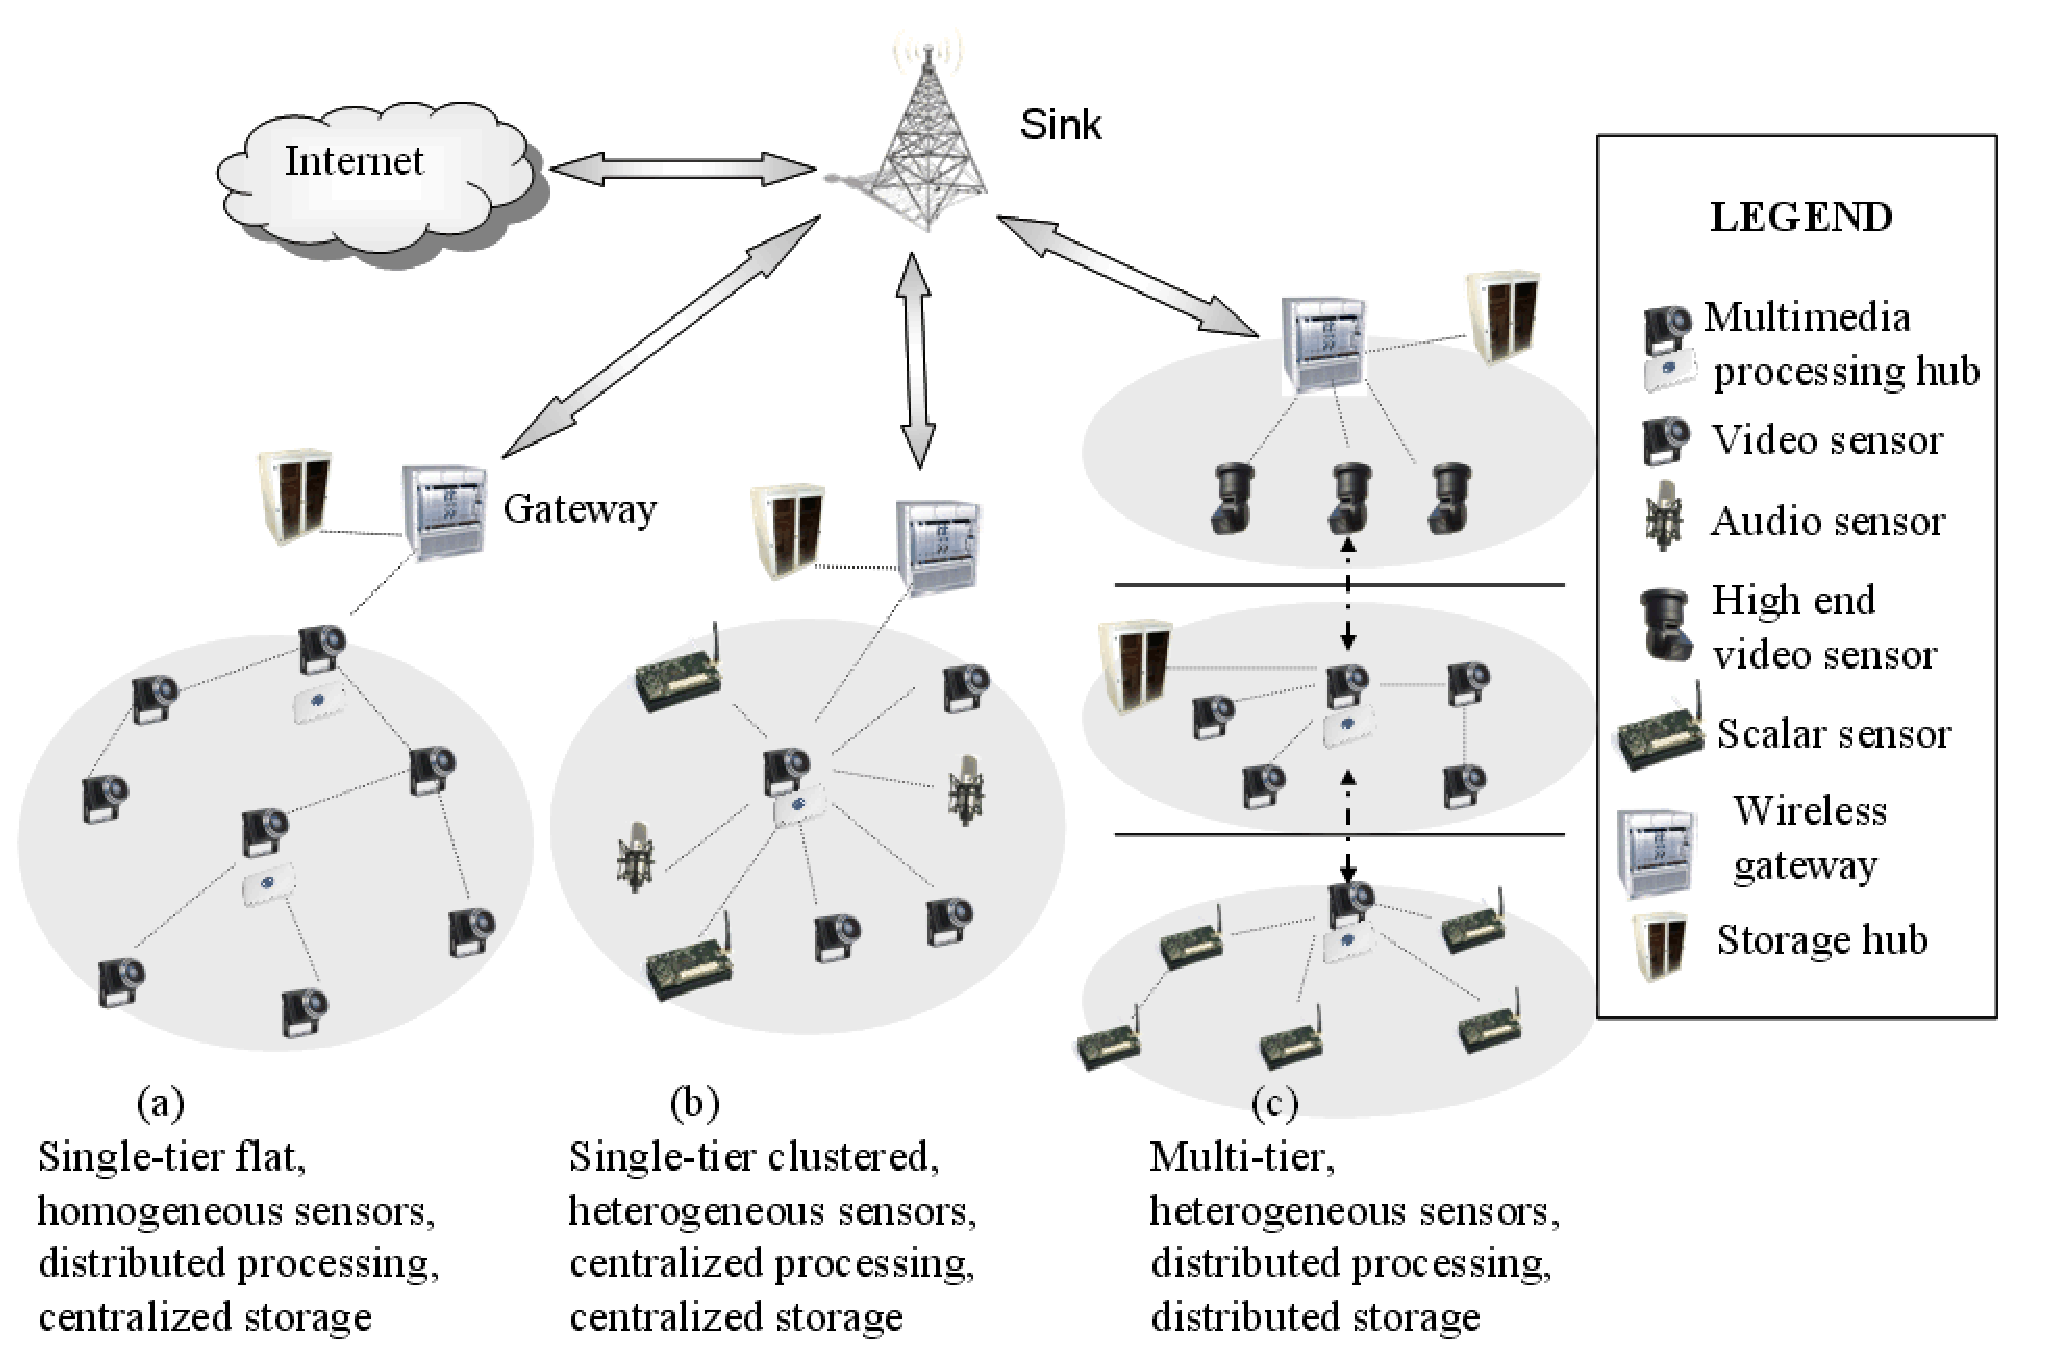
\includegraphics[width=13cm]{pictures/WMSN}
\caption[Esempio di WMSN]{Esempio di architettura di una \textit{wireless multimedia sensor network} (WMSN)}
\label{fig:WMSN}
\end{figure}
Questi particolari nodi prendono il nome di \textit{smart camera}, o camere intelligenti \cite{wolf2002smart}, e sono dispositivi che integrano al loro interno \textit{camere digitali}, \textit{capacit\`a di calcolo} e \textit{interfacce di rete}.
In questo modo \`e possibile eseguire algoritmi di elaborazione di immagini o di visione artificiale direttamente sul dispositivo, e ottenere un'\textit{intelligenza distribuita} su tutta la rete.
Il fatto di poter eseguire degli algoritmi direttamente sul dispositivo che acquisisce i dati, inoltre, permette di ridurre il consumo energetico limitando il traffico dei dati sulla rete.\\
Gli scenari pi\`u interessanti di impiego delle MSSN sono quelli in cui non si pu\`o avere accesso alla rete elettrica per alimentare i sensori: questo pu\`o accadere, ad esempio, nel caso in cui si voglia monitorare, con una copertura capillare, ambienti esterni, o pi\`u in generale vaste aree extra urbane in cui non \`e possibile allacciarsi alla rete elettrica.\\
La necessit\`a di operare in ambienti privi di energia elettrica richiede nodi alimentati a \textit{batteria} in grado di garantire l'operabilit\`a delle camere per degli anni.
%
%Questo pone il problema di avere dei nodi alimentati a \textit{batteria} che possano mantenere la carica a lungo, anche degli anni.
Lo sviluppo di camere intelligenti a \textit{basso consumo energetico} \`e gi\`a in atto, e sono gi\`a presenti dei prototipi o prodotti commerciali.
\textit{STMicroelectronics} ha sviluppato una smart camera in grado di acquisire e trasmettere immagini e video, e fare semplici elaborazioni sui frame, come ad esempio identificazione di oggetti o classificatori.
La corrente assorbita da questo dispositivo \`e di circa $30-40 \mu \text{A}$, a circa $1.2-1.5 \text{V}$.
Questo vuol dire che, utilizzando due batterie di tipo AA per alimentare il dispositivo, la loro carica potrebbe mantenersi per degli \textit{anni}.
Questa ottimizzazione del consumo di energia \`e dovuta innanzitutto alla possibilit\`a di integrare degli algoritmi direttamente in \textit{hardware}.
%Inoltre, dato che la trasmissione delle immagini sulla rete richiede molta energia, è auspicabile un elaborazione locale per determinare se vale la pena accendere la radio e trasmettere.
Un altro fattore che determina il consumo della batteria \`e il \textit{contesto applicativo} in cui la camera opera.
Ad esempio, il \textit{framerate}, ovvero la frequenza con cui la camera acquisisce le immagini, ha degli impatti molto alti sul consumo di potenza del dispositivo.
Per alcune applicazioni di monitoraggio video potrebbe non essere necessario avere un'acquisizione \textit{continua}, ovvero tra i $30$ e i $2$ \textit{frame per secondo} (fps), da parte della camera, ma basterebbe un'acquisizione ed elaborazione a framerate molto pi\`u bassi, ad esempio un frame ogni minuto.\\
%A volte per le finalit\`a per cui si colloca la telecamera potrebbe non servire l'acquisizione a 30fps ma basterebbe un'acquisizione ed un'elaborazione a framerate molto più bassi, ad esempio 1 frame al minuto. Eventualmente aggiungendo che la trasmissione dei dati sulla rete richiede molta energia e quindi un processing locale per determinare se vale la pena accendere la radio e trasmette è auspicambile.
%Acquisire $30$ frame ogni secondo, per esempio, fa consumare al dispositivo molta pi\`u corrente rispetto ad acquisire un frame ogni minuto.\\
%
%questo è un po' banale. Girerei il problema nel seguente modo: a volte per le finalità per cui si colloca la telecamera potrebbe non servire l'acquisizione a 30fps ma basterebbe un'acquisizione ed un'elaborazione a framerate molto più bassi, ad esempio 1 frame al minuto. Eventualmente aggiungendo che la trasmissione dei dati sulla rete richiede molta energia e quindi un processing locale per determinare se vale la pena accendere la radio e trasmette è auspicambile.
%
%In generale, uno potrebbe dire.. beh ma che applicazioni girano su questa camera che acquisice ad 1frame al minuto e che uno potrebbe manomettere? Questa è una cosa da chiarire, dicendo che l'acquisizione potrebbe essere di default a basso framerate (sotto 1 fps) ed eventualmente triggerata da altri sensori del dispositivo (es sensori di prossimtà) o da altri dispositivi nella rete.
In questo lavoro di tesi affrontiamo un particolare problema legato ai sistemi di monitoraggio video, e consideriamo il caso particolare in cui vengano impiegate camere intelligenti a basso consumo energetico.\\
Uno dei maggiori problemi quando si ha a che fare con sistemi di monitoraggio video consiste nell'identificazione di eventi in grado di compromettere la corretta ripresa della scena da parte del sensore.
Eventi di questo tipo sono, ad esempio, lo spostamento della camera, oppure il cambio di messa a fuoco della scena.\\
Questo tipo di eventi viene classificato generalmente sotto il nome di \textit{tampering}, dall'inglese \textit{manomissione}.
Il termine deriva dal fatto che, di solito, questi eventi sono legati ad azioni intenzionali atte a impedire che la camera riprenda correttamente la scena.
Pu\`o succedere, ad esempio, che un ladro copra l'obiettivo della camera con qualche oggetto, in modo da poter agire indisturbato, oppure che la sposti in modo che riprenda qualcos'altro.
\begin{figure}
	\centering
	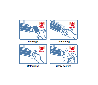
\includegraphics[width=7cm]{pictures/tamperdetection}
	\caption[Esempi di eventi di tampering intenzionali]{Esempi di eventi di tampering intenzionali. Per evitare che la camera riprenda correttamente la scena \`e possibile coprire il sensore con un oggetto opaco, oppure spostarla in modo che riprenda una scena diversa. Altre manomissioni possono essere fatte cambiando la messa a fuoco della camera o spruzzando della vernice spray sull'obiettivo.}
	\label{fig:tamperdetection}
\end{figure}
Esempi di tampering intenzionale sono illustrati nella Figura \ref{fig:tamperdetection}.
In questa tesi definiamo con il termine tampering un qualsiasi evento, intenzionale o meno, che possa compromettere la corretta acquisizione della scena inquadrata dalla camera.
Ad esempio una sfocatura pu\`o essere causata da dell'acqua piovana che si deposita a ridosso della lente, oppure pu\`o succedere che una folata di forte vento sposti la camera, cambiando quindi l'inquadratura della scena, oppure che della neve si depositi sulla camera e non permetta di vedere parte della scena.
Esempi di eventi di tampering dovuti a cause naturali sono illustrati nella Figura \ref{fig:tamperingNaturali}.\\
Il problema di individuare, in maniera automatica, eventi di tampering, sia intenzionali che dovuti a cause naturali, prende il nome di \textit{tampering detection}.
\begin{figure}[tb]
	\centering
	\begin{subfigure}[]
		{\label{fig:pioggia1} 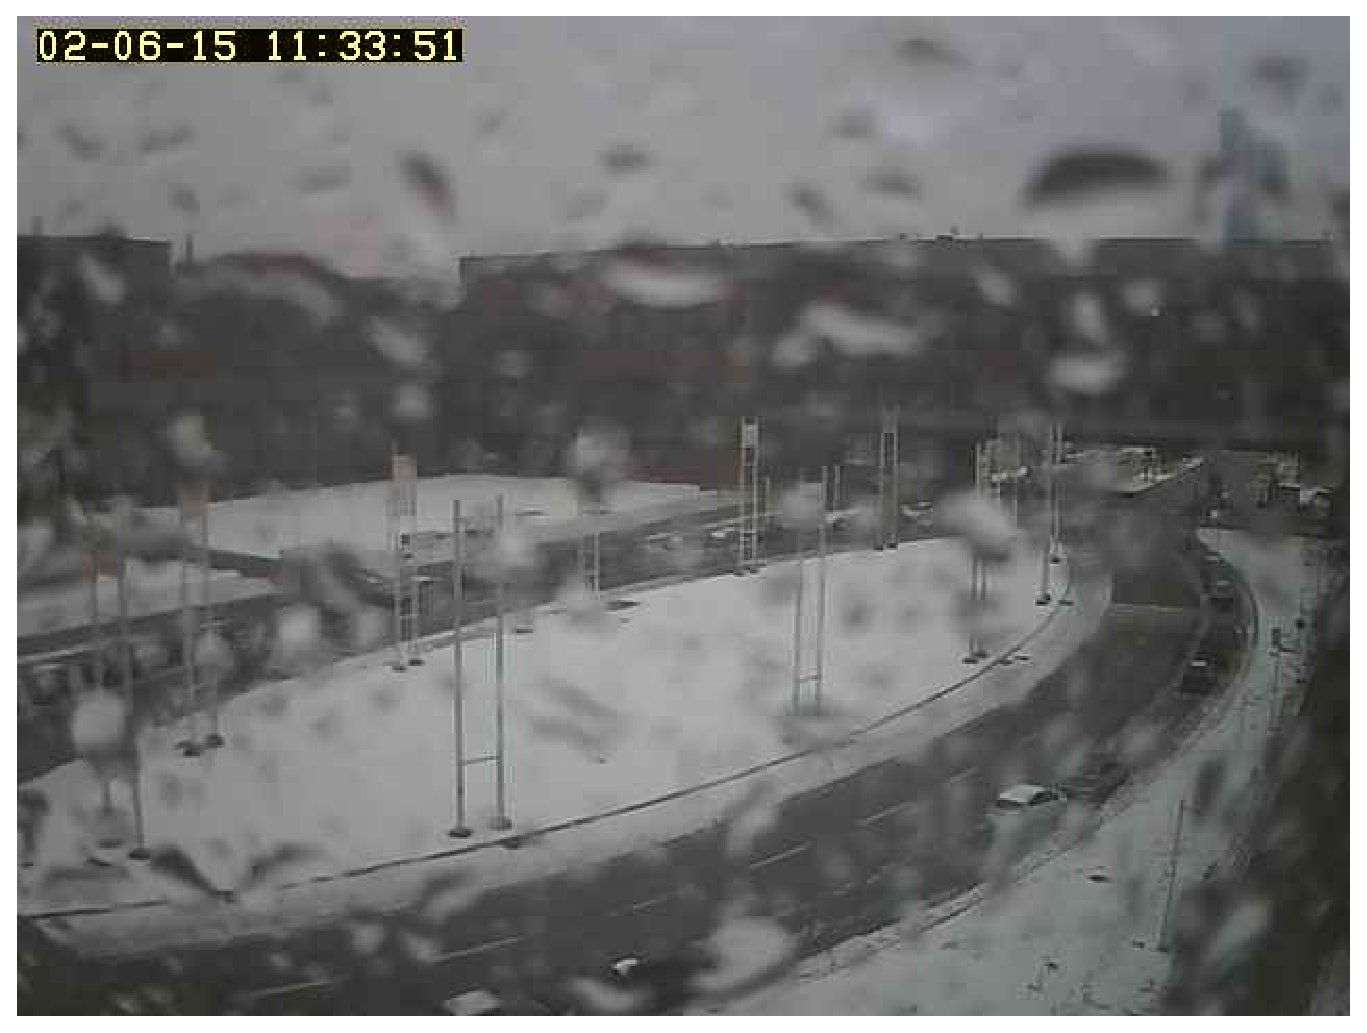
\includegraphics[width=6cm]{./pictures/pioggia}}
	\end{subfigure}
	\begin{subfigure}[]
		{\label{fig:neve1} 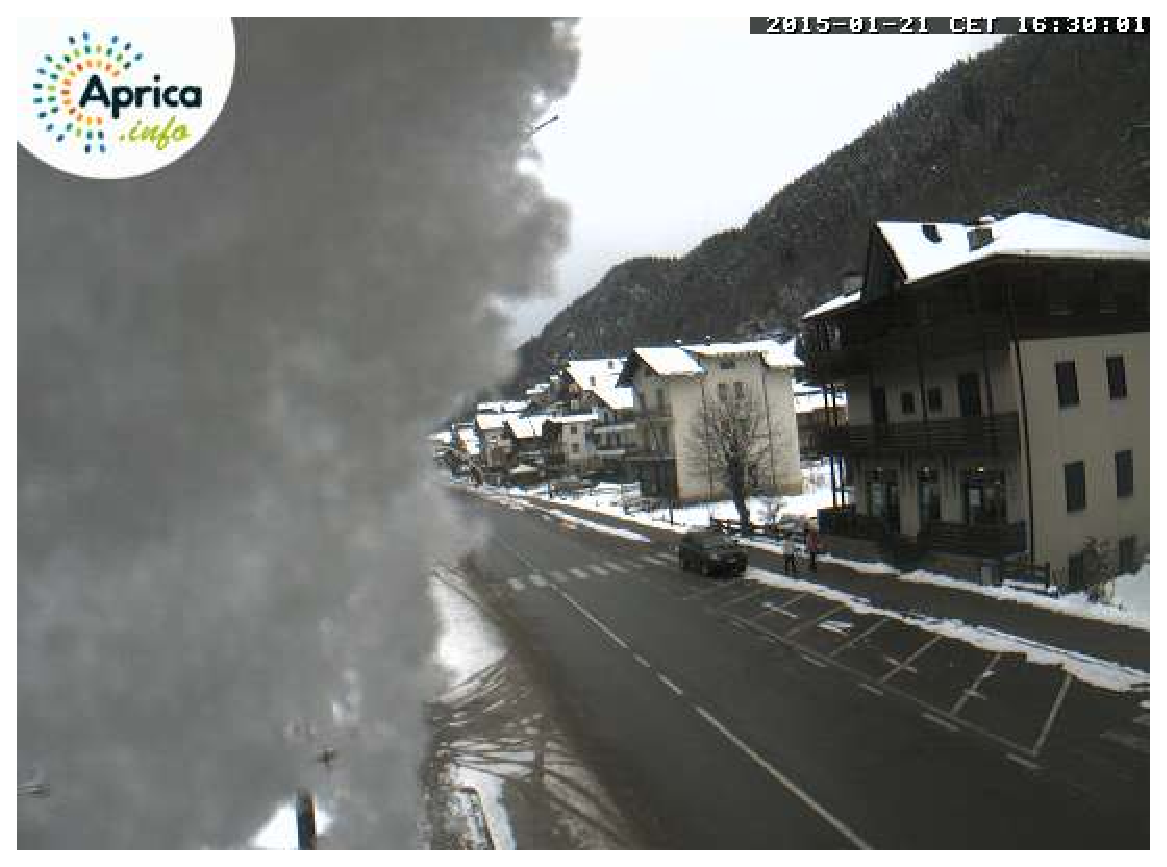
\includegraphics[width=6cm]{./pictures/neve}}
	\end{subfigure}
	\caption[Esempi di eventi di tampering dovuti a cause naturali]{Esempi di eventi di tampering dovuti a cause naturali: in (a) vediamo come le gocce di pioggia possano portare a delle sfocature nell'immagine, con la conseguente perdita di dettagli, mentre in (b) possiamo vedere un cumulo di neve sulla camera che impedisce di riprendere la totalit\`a della scena.}
	\label{fig:tamperingNaturali}
\end{figure}
La letteratura scientifica ha prodotto molte soluzioni a riguardo \cite{harasse2004automated,aksay2007camera,saglam2009real,ellwart2012camera,tsesmelis2013tamper}, ma la maggior parte sono legate ad applicazioni in cui le camere operano a framerate \textit{continuo}, solitamente tra i 30 frame per secondo (fps) e i 2 fps.
Utilizzando frequenze di acquisizione cos\`i alte abbiamo frame consecutivi molto simili fra loro anche in scene molto dinamiche, in cui non avvengono cambiamenti sostanziali all'interno della scena ripresa, a meno di eventi di tampering.
Ci\`o permette di utilizzare tecniche di \textit{background subtraction} o di confronto tra frame consecutivi, e quindi rilevare l'evento di tampering come un cambiamento sostanziale della scena.
Queste tecniche, oltre a richiedere capacit\`a di calcolo e di memoria che una camera a basso consumo di potenza difficilmente pu\`o garantire, risultano essere non efficaci nel caso in cui la frequenza con cui i frame vengono acquisiti \`e bassa.
Infatti, in questo caso, le differenze tra due immagini acquisite consecutivamente sono molto elevate, in quanto elementi come i \textit{cambiamenti di luminosit\`a} e la \textit{dinamicit\`a} della scena sono pi\`u marcati rispetto al caso di acquisizione continua.\\
Lo scopo della tesi \`e lo sviluppo di un algoritmo di tampering detection per camere intelligenti (\textit{smart camera}) e a basso consumo, in cui si opera a framerate bassi, minori di 1fps.
Lo sviluppo dell'algoritmo \`e stato fatto nell'ottica di mantenere al minimo il numero di falsi allarmi lanciati dal sistema.
Questi ultimi, infatti, comportano un costo dal punto di vista del consumo energetico, in quanto vengono trasmessi sulla rete dei segnali di allarme non necessari.\\
La soluzione che proponiamo \`e quella di monitorare degli indicatori a basso costo computazionale, estratti dalle singole immagini, in modo da identificare l'istante in cui avviene l'evento di tampering.
Le tecniche di monitoraggio utilizzate sono due:
\begin{itemize}
	\item \textbf{one-shot}, in cui verifichiamo che il valore dell'indicatore, in ogni istante, stia all'interno di un intervallo definito da due \textit{soglie}, calcolate a partire da un insieme di osservazioni di \textit{training};
	\item \textbf{sequenziale}, in cui verifichiamo la \textit{stazionariet\`a} dell'indicatore nel tempo, ovvero l'ipotesi che le osservazioni siano \textit{indipendenti e identicamente distribuite} (i.i.d.).
\end{itemize}
Per garantire alte prestazioni e limitare il numero di falsi allarmi, abbiamo deciso di applicare questo monitoraggio su alcune \textit{regioni adattative} estratte dalla scena.
%Questi indicatori, per\`o, non sono definiti su tutta l'immagine, ma su \textit{regioni adattative} estratte dalla scena.
A questo scopo abbiamo sviluppato un \textit{algoritmo di segmentazione} che permetta di estrarre queste regioni.
Questo algoritmo viene eseguito durante la configurazione del sistema, separatamente rispetto alla fase di identificazione degli eventi di tampering.
La segmentazione, quindi, non comporta ulteriore costo computazionale all'algoritmo, in cui viene considerata semplicemente come una variabile d'ingresso.
Inoltre, la segmentazione pu\`o essere eseguita \textit{offline} su un dispositivo esterno come una centrale operativa o un pc collegato alla smart camera durante la fase di configurazione della rete.\\
Per validare le nostre scelte abbiamo implementato la nostra soluzione in MATLAB %, un ambiente per il calcolo numerico e l'analisi statistica, che dispone di numerose librerie per l'elaborazione di segnali e immagini, 
e fatto degli esperimenti su alcuni \textit{dataset} di sequenze video con la presenza di eventi di tampering, sia sintetici che reali.
Gli esperimenti condotti hanno confermato come l'utilizzo della segmentazione della scena porti a dei miglioramenti nelle prestazioni dell'algoritmo, diminuendo il numero di falsi allarmi.\\
La tesi \`e stata svolta durante un lavoro di stage presso la divisione \textit{Advanced System Technology} di \textit{STMicroelectronics}, collaborando in particolare con un gruppo dove la ricerca \`e volta allo sviluppo di algoritmi intelligenti di elaborazione immagini da integrare nei propri dispositivi embedded.\\
%Una branca dell'industria tecnologica che sta prendendo sempre pi\`u piede \`e quella dei \textit{sistemi di monitoraggio video}.
%L'abbattimento dei costi delle camere e una sempre maggiore integrazione di tecnologie hardware con sensori e infrastrutture di rete hanno permesso una rapida crescita di questo settore.\\
%Inoltre, il grande successo di Internet degli ultimi anni ha permesso l'utilizzo dei sistemi di monitoraggio video per applicazioni che prima non erano neanche pensabili.
%Oggigiorno \`e possibile avere un sistema di videosorveglianza domestico spendendo poche centinaia di euro, controllabile con il proprio \textit{smartphone} attraverso Internet, oppure \`e possibile vedere le condizioni meteorologiche o del traffico nella propria citt\`a attraverso le immagini riprese da una \textit{webcam}.
%Un servizio di questo genere \`e fornito da molte piattaforme web di previsioni del tempo.
%Ad esempio, il sito \textit{ilMeteo.it} \cite{ilmeteo} permette di vedere in tempo reale il contenuto video di webcam presenti nelle principali citt\`a o in localit\`a di interesse turistico.\\
%Uno dei maggiori problemi quando si ha a che fare con sistemi di monitoraggio video consiste nell'identificazione di particolari eventi in grado di compromettere la corretta ripresa della scena da parte del sensore.\\
%%Eventi di questo tipo sono, ad esempio, lo spostamento della camera, oppure una scorretta messa a fuoco della scena.\\
%Questo tipo di eventi viene classificato generalmente sotto il nome di \textit{tampering}, dall'inglese \textit{manomissione}.
%Il termine deriva dal fatto che, di solito, questi eventi sono legati ad azioni intenzionali atte a impedire che la camera riprenda correttamente la scena.
%Pu\`o succedere, ad esempio, che un ladro copra l'obiettivo della camera con qualche oggetto, in modo da poter agire indisturbato, oppure che la sposti in modo che riprenda qualcos'altro.
%In questa tesi definiamo con il termine tampering un qualsiasi evento, intenzionale o meno, che possa compromettere la corretta acquisizione della scena inquadrata dalla camera.
%Ad esempio una sfocatura pu\`o essere causata da dell'acqua piovana che si deposita a ridosso della lente, oppure pu\`o succedere che una folata di forte vento sposti la camera, cambiando quindi l'inquadratura della scena.\\
%Questa definizione permette di analizzare il problema anche per quelle applicazioni di monitoraggio video che non sono direttamente legate alla videosorveglianza, ad esempio per lo scenario delle webcam introdotto sopra, in cui l'evento non \`e necessariamente dovuto a un intervento umano intenzionale.\\
%Le tecniche algoritmiche che vengono utilizzate per identificare gli eventi di tampering prendono il nome di algoritmi di \textit{tampering detection}.\\
%La letteratura scientifica ha prodotto molte soluzioni a riguardo, ma la maggior parte sono legate ad applicazioni di videosorveglianza.
%Questo particolare tipo di applicazioni ha bisogno di camere che acquisiscano a framerate \textit{continuo}, solitamente tra i 30 frame per secondo (fps) e i 2 fps.
%\`E infatti impensabile che una camera di videosorveglianza possa acquisire, ad esempio, un frame ogni minuto.\\
%Lo scopo della tesi \`e lo sviluppo di un algoritmo di tampering detection per camere intelligenti (\textit{smart camera}) e a basso consumo.
%In particolare abbiamo considerato scenari in cui la camera operi a \textit{basso framerate}, ad esempio acquisendo un'immagine ogni minuto.\\
%Questa assunzione copre in realt\`a molti casi d'uso gi\`a esistenti, che non sono legati alla videosorveglianza.
%\begin{figure}[t]
%	\centering
%	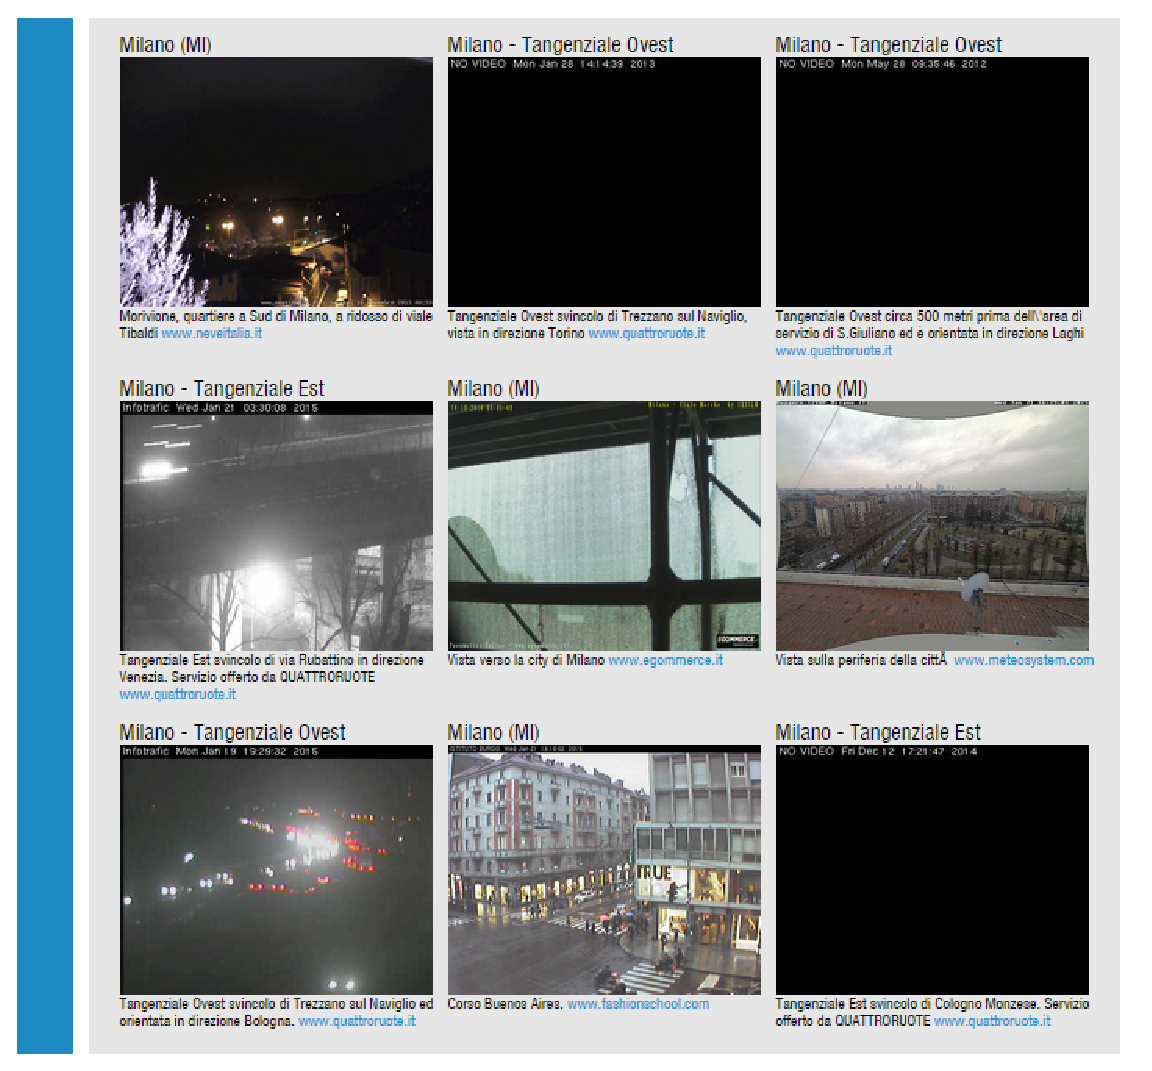
\includegraphics[width=12cm]{pictures/ilMeteo}
%	\caption[Webcam per il monitoraggio meteorologico]{In questa figura vediamo un esempio di applicazione per sistemi di monitoraggio video. Molti siti di previsioni del tempo consentono l'accesso alle immagini registrate da webcam utilizzate per il monitoraggio meteorologico. Come possiamo vedere, la webcam al centro dell'immagine non \`e in condizioni di riprendere correttamente la scena, in quanto c'\`e un'impalcatura che ne impedisce la visione. Inoltre, possiamo vedere come alcune webcam non riprendano alcuna scena.}
%	\label{fig:ilMeteo}
%\end{figure}
%Un esempio \`e quello delle webcam per il monitoraggio meteorologico che abbiamo illustrato precedentemente.
%Nella Figura \ref{fig:ilMeteo} possiamo vedere come una parte delle webcam accessibili da un sito di previsioni del tempo in realt\`a non forniscano molte informazioni riguardanti il monitoraggio meteorologico:
%alcune webcam sono spente, e quindi non inviano frame alla piattaforma, e una camera, quella centrale, non pu\`o riprendere la scena perch\'e le \`e stata posta un'impalcatura davanti.
%Avere delle tecniche in grado di identificare in maniera automatica questo tipo di eventi potrebbe evitare l'invio di immagini compromesse e inviare un segnale di allarme al gestore della camera, che provvederebbe alla risoluzione del problema, ad esempio cambiando la locazione della camera.
%In questo modo si aumenterebbe l'affidabilit\`a del sistema e si diminuirebbe il traffico di dati sulla rete, in quanto si eviterebbe di inviare frame compromessi.\\
%
%Le tecniche principalmente utilizzate nella letteratura scientifica hanno come base il confronto di ciascun frame con quelli successivi, utilizzando \textit{modelli di background}.
%Queste, per essere efficaci, hanno bisogno che i frame vengano acquisiti a framerate continuo, in quanto viene fatta l'ipotesi che tra i vari frame della scena il contenuto vari poco.
%Abbiamo notato, invece, che operando a basso framerate le differenze tra frame consecutivi sono molto elevati, a causa di cambiamenti di luminosit\`a, di ombre e di zone dinamiche della scena.\\
%Il nostro lavoro di tesi \`e una prosecuzione del lavoro svolto da \cite{alippi2010detecting}, dove vengono identificati eventi di sfocatura utilizzando \textit{tecniche sequenziali} su un indicatore \textit{scalare} estratto da ciascun frame.\\
%Il nostro lavoro si \`e concentrato sugli eventi di \textit{sfocatura} e di \textit{spostamento della camera}.
%Per individuare questi eventi analizziamo il comportamento di indicatori scalari estratti dalle singole immagini.
%Abbiamo notato come questi eventi determinino un cambiamento molto brusco nel normale andamento di questi indicatori.


\noindent La tesi \`e strutturata nel seguente modo.\\
Nel Capitolo \ref{StatoArte} illustriamo le principali tecniche di identificazione di tampering presenti nella letteratura scientifica, introducendo anche alcuni principi di visione artificiale e di elaborazione di immagini necessari alla comprensione del resto della trattazione.\\
Nel Capitolo \ref{FormulazioneProblema} diamo una definizione formale degli eventi di tampering e del problema che si pone l'algoritmo di tampering detection.\\
Nel Capitolo \ref{SoluzioneProposta} illustriamo la soluzione che abbiamo proposto in questa tesi per il problema dell'identificazione degli eventi di tampering, entrando nel merito sui dettagli realizzativi.\\
Nel Capitolo \ref{ProveSperimentali} mostriamo le prove realizzate per validare la soluzione proposta, descrivendo anche le procedure di acquisizione, la preparazione dei dataset e i risultati ottenuti.\\
Nel Capitolo \ref{Conclusioni}, infine, presentiamo le considerazioni conclusive e le prospettive future di ricerca.
	
